% Options for packages loaded elsewhere
\PassOptionsToPackage{unicode}{hyperref}
\PassOptionsToPackage{hyphens}{url}
%
\documentclass[
  11pt,
  a4paper,
]{article}
\usepackage{amsmath,amssymb}
\usepackage{lmodern}
\usepackage{iftex}
\ifPDFTeX
  \usepackage[T1]{fontenc}
  \usepackage[utf8]{inputenc}
  \usepackage{textcomp} % provide euro and other symbols
\else % if luatex or xetex
  \ifXeTeX
    \usepackage{zxjatype} 
    \usepackage[ipaex]{zxjafont}
    \setromanfont{Times New Roman}
  \fi
  \usepackage{unicode-math}
  \defaultfontfeatures{Scale=MatchLowercase}
  \defaultfontfeatures[\rmfamily]{Ligatures=TeX,Scale=1}
\fi
% Use upquote if available, for straight quotes in verbatim environments
\IfFileExists{upquote.sty}{\usepackage{upquote}}{}
\IfFileExists{microtype.sty}{% use microtype if available
  \usepackage[]{microtype}
  \UseMicrotypeSet[protrusion]{basicmath} % disable protrusion for tt fonts
}{}
\usepackage{xcolor}
\IfFileExists{xurl.sty}{\usepackage{xurl}}{} % add URL line breaks if available
\IfFileExists{bookmark.sty}{\usepackage{bookmark}}{\usepackage{hyperref}}
\hypersetup{
  pdftitle={Appendix ``Text-Based Nudges Promoting Rubella Antibody Testing and Vaccination: Evidence from Nationwide Online Field Experiment in Japan''},
  hidelinks,
  pdfcreator={LaTeX via pandoc}}
\urlstyle{same} % disable monospaced font for URLs
\usepackage[left=3cm,right=3cm,top=3cm,bottom=3cm]{geometry}

\usepackage{setspace}
\renewcommand{\baselinestretch}{1.5}
\usepackage{float}

\usepackage{longtable,booktabs,array}
\usepackage{threeparttable, threeparttablex, multirow}
\usepackage{calc} % for calculating minipage widths
% Correct order of tables after \paragraph or \subparagraph
\usepackage{etoolbox}
\makeatletter
\patchcmd\longtable{\par}{\if@noskipsec\mbox{}\fi\par}{}{}
\makeatother
% Allow footnotes in longtable head/foot
\IfFileExists{footnotehyper.sty}{\usepackage{footnotehyper}}{\usepackage{footnote}}
\makesavenoteenv{longtable}
\usepackage{graphicx}
\makeatletter
\def\maxwidth{\ifdim\Gin@nat@width>\linewidth\linewidth\else\Gin@nat@width\fi}
\def\maxheight{\ifdim\Gin@nat@height>\textheight\textheight\else\Gin@nat@height\fi}
\makeatother
% Scale images if necessary, so that they will not overflow the page
% margins by default, and it is still possible to overwrite the defaults
% using explicit options in \includegraphics[width, height, ...]{}
\setkeys{Gin}{width=\maxwidth,height=\maxheight,keepaspectratio}
% Set default figure placement to htbp
\makeatletter
\def\fps@figure{htbp}
\makeatother
\setlength{\emergencystretch}{3em} % prevent overfull lines
\providecommand{\tightlist}{%
  \setlength{\itemsep}{0pt}\setlength{\parskip}{0pt}}
\setcounter{secnumdepth}{5}


\usepackage{float}
\usepackage{threeparttable}
\ifLuaTeX
  \usepackage{selnolig}  % disable illegal ligatures
\fi

\makeatletter
\def\@fnsymbol#1{\ensuremath{\ifcase#1\or \dagger\or \ddagger\or
   \mathsection\or \mathparagraph\or \|\or **\or \dagger\dagger
   \or \ddagger\ddagger \else\@ctrerr\fi}}
    \makeatother
\title{Appendix
``Text-Based Nudges Promoting Rubella Antibody Testing and Vaccination:
Evidence from Nationwide Online Field Experiment in Japan''  }

\date{2022/07/01}



\begin{document}
\begin{spacing}{1}
  \maketitle
\end{spacing}

{
\setcounter{tocdepth}{2}
\tableofcontents
}
\clearpage

\hypertarget{appendix-appendix}{%
\appendix}


\hypertarget{background-on-routine-rubella-vaccination-in-japan}{%
\section{Background on Routine Rubella Vaccination in Japan}\label{background-on-routine-rubella-vaccination-in-japan}}

ワクチン接種は、
予防接種法(Immunization Act)で規定されている定期接種(routine vaccination)と
それ以外の任意接種(voluntary vaccination)がある。
定期接種は原則として自己負担がないが、任意接種は接種料金を自己負担する必要がある。

感染予防効果を持つ風しんワクチンは、妊婦の感染防止のために1977年8月から定期接種の対象となった。
対象者は中学生の女子であり、1回の定期接種を義務として課された。
同時に、1989年4月から、生後12-72カ月の幼児が麻疹ワクチンの定期接種を受けるとき、
親は麻しん・おたふくかぜ・風しん混合ワクチン(MMRワクチン)を選択することができた。
しかしながら、無菌性髄膜炎(aseptic meningitis)をもたらすために、
MMRワクチンの定期接種は1993年4月に一旦中止された。

1994年の予防接種方の改正により、定期接種は義務接種ではなく、努力義務となった。
これに伴い、1995年4月から、風しんワクチンの定期接種の対象者は生後12-90ヵ月未満の男女に変わった。
これは風しんの流行そのものを止めるために集団免疫(herd immunity)の獲得を目的としている。
また、それ以前に風しんワクチンやMMRワクチンを接種していない人々に対して経過措置(transitional measures)が取られた。
経過措置の定期接種の対象者は
(1)1995年度に小学校1-2年生と生後90カ月未満の男女、
(2)1996-1999年度に小学校1年生、
(3)1995年4月から2003年9月にかけて、1979年4月2日から1987年10月1日に生まれた中学生男女である。

2006年から、麻疹風しん混合ワクチン(MRワクチン)を用いて、2回の定期接種が行われている。
1回目は生後12-24カ月の幼児期であり、2回目は小学校入学前1年間の幼児期である。
さらに、2007年から始まった10代・20代を中心とする麻疹の全国的な流行を受けて、
2008年4月から2013年3月までにかけて、
当時中学1年生および高校3年生相当の学生を対象に、MRワクチンの2回目接種の機会が設けられた。

以上で述べた定期接種の歴史的な背景の結果、
日本では風しんワクチンの定期接種を受けていない2つの年齢層が生じることになった。
定期接種を受けていない世代は、
(1)1962年4月2日以前に生まれた男女と
(2)1962年4月2日から1979年4月1日に生まれた男性である。
前者のグループは1977年の風しんワクチンの定期接種が始まる前に中学校を卒業している。
後者のグループは風しんワクチンの定期接種の対象が中学生女子であり、1995年以降の経過措置の対象にならなかった。
1979年4月2日以降に生まれた男女は経過措置を含めて定期接種の対象者となっているが、接種回数は年齢によって異なる。
定期接種を受けていない人は自然感染による抗体保有の可能性があるだけで、ワクチン接種による風しん抗体を保有していない。

本論で述べたように、
定期接種を受けていない二つの世代のうち、
前者のグループは風しんが流行していた期間に育っているので、感染を通じて抗体を保有している可能性が高い。
したがって、2019年4月から、厚生労働省は1962年4月2日から1979年4月1日に生まれた男性を対象として、
風しんワクチンの定期接種の追加対策を実行した。
この追加対策の政策目標は2022年3月までに対象世代の男性の抗体保有率を80\%から90\%に引き上げることである。
この目標が達成されれば、日本は風しんの集団免疫を獲得できる。

\begin{figure}[t]
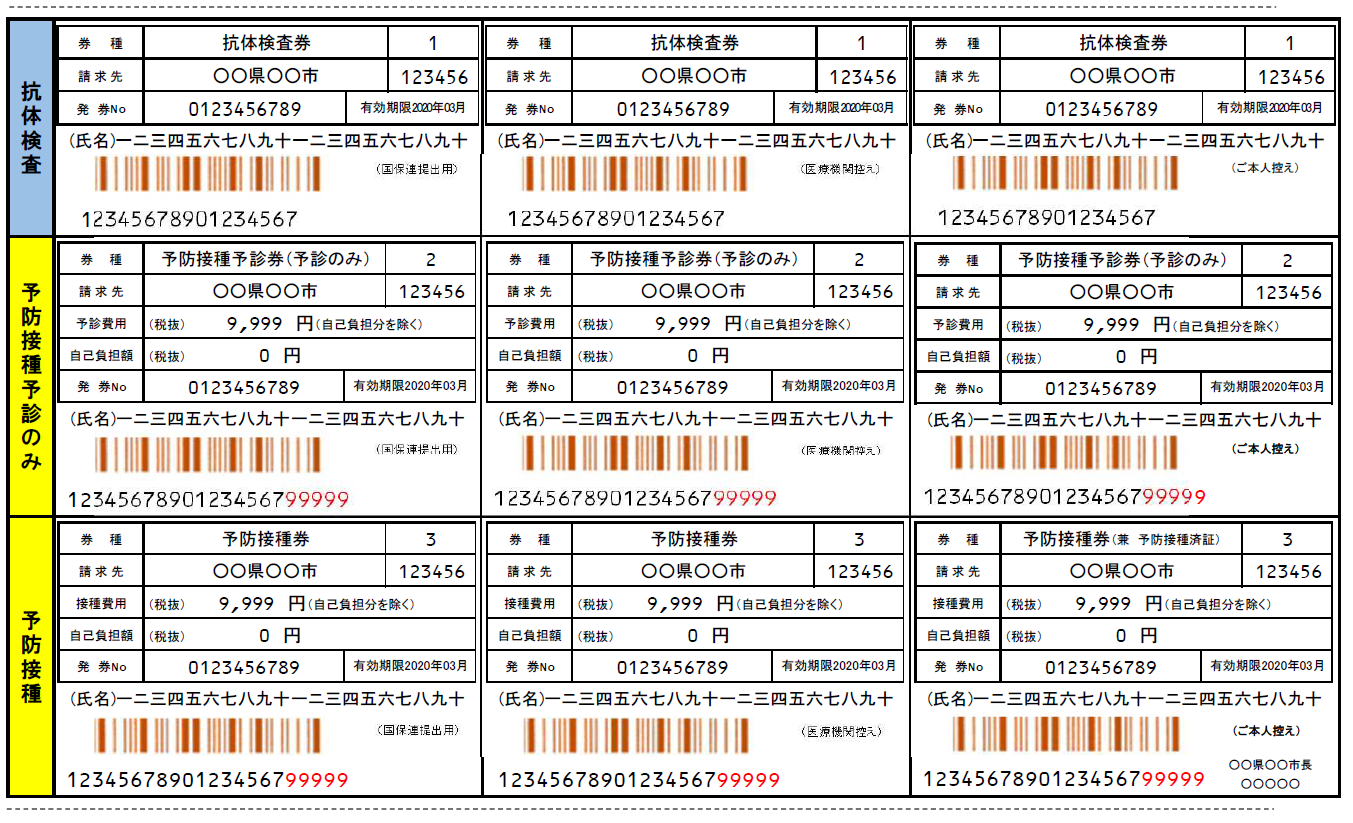
\includegraphics[width=1\linewidth]{C:/Users/vge00/Desktop/MHLW-Rubella-Project/2020-online-RCT/assets/rubella-coupon} \caption{Sample Coupon for Free Rubella Antibody Test and Vaccination}\label{fig:coupon}
\end{figure}

この追加対策で、対象の男性は風しんの抗体検査とワクチン接種を無料で受けられる
クーポン券を地方自治体から送付される(図\ref{fig:coupon})。
このクーポン券を利用して、対象者は抗体検査を受検する。
抗体検査によって抗体を保有していないことが明らかになれば、
対象者は風しんワクチンを無料でう接種できる。

\clearpage

\hypertarget{additional-tables-and-figures-about-online-survey-experiment}{%
\section{Additional Tables and Figures about Online Survey Experiment}\label{additional-tables-and-figures-about-online-survey-experiment}}

\begin{figure}[t]
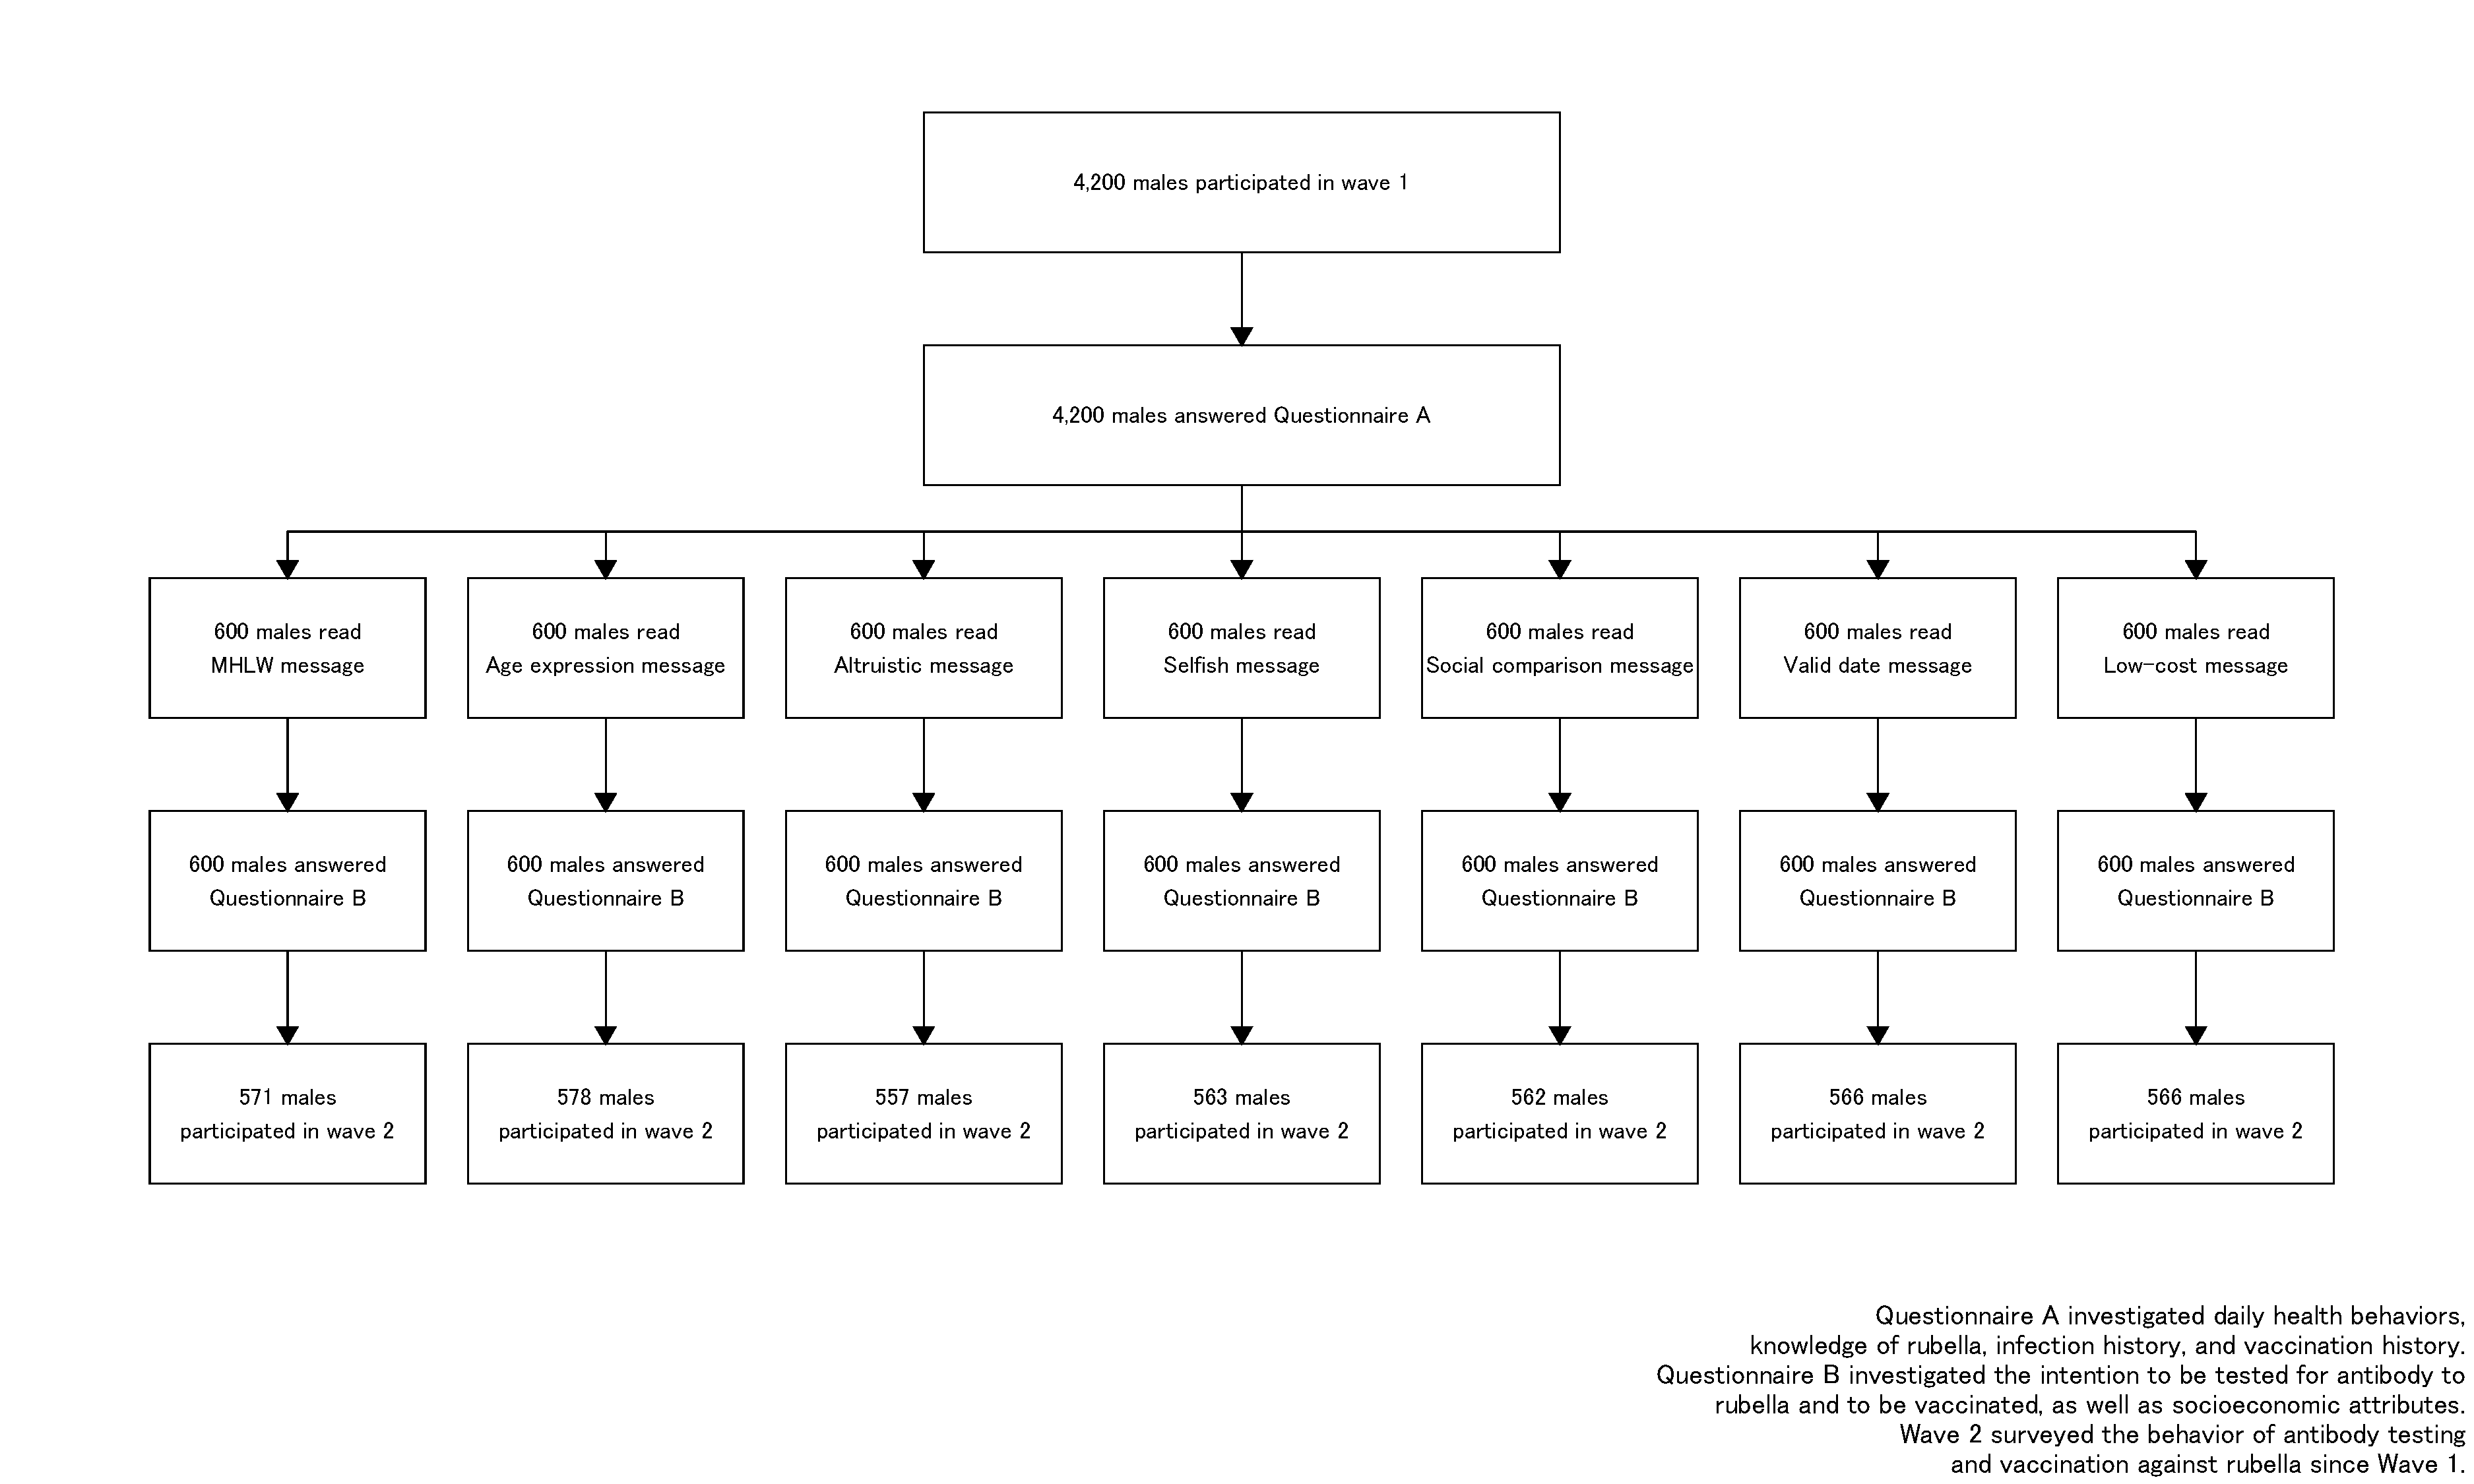
\includegraphics[width=1.5\linewidth,angle=90]{C:/Users/vge00/Desktop/MHLW-Rubella-Project/2020-online-RCT/publish/appendix_files/figure-latex/flowchart-1} \caption{Overview of Online Survey Experiment}\label{fig:flowchart}
\end{figure}

本研究が実施したオンライン調査の概要を説明する。
我々はインターネット調査会社であるマイボイスコム株式会社(MyVociceCome Co.~Ltd.)に委託し、
2回のオンライン調査を実施した。
図\ref{fig:flowchart}に調査の流れを示した。

\begin{table}[!h]

\caption{\label{tab:covlist}List of Covariates}
\centering
\fontsize{9}{11}\selectfont
\begin{tabular}[t]{l>{\raggedright\arraybackslash}p{30em}cc}
\toprule
  & Description & Mean & Std.Dev.\\
\midrule
age & (Wave1) Age as of April 2019 based on year of birth and month of birth. & 48.66 & 5.69\\
coupon2019 & (Wave1) Dummy variable taking one if 40 to 46 years old as of April 2019. & 0.35 & 0.48\\
married & (Wave1) Dummy variable taking one if a respondent is married. & 0.58 & 0.49\\
education & (Wave1) Years of education. & 14.75 & 2.31\\
exercise\_w1 & (Wave1) Dummy variable taking one if a respondent exercises or plays sports more than once a week. & 0.22 & 0.42\\
health\_check & (Wave1) Dummy variable taking one if a respondent has had medical examination at his/her city or place of employment in the past year from the time of the wave 1. & 0.68 & 0.46\\
flushot & (Wave1) Dummy variable taking one if a respondent is vaccinated against influenza every year. & 0.27 & 0.45\\
handwash & (Wave2) Five Likert scale for the question "I wash my hands and gargle frequently during the period from the end of the previous questionnaire response to today." & 3.91 & 1.04\\
temp\_check & (Wave2) Five Likert scale for the question "I take my tempature frequently during the period from the end of the previous questionnaire response to today." & 2.26 & 1.22\\
avoid\_out & (Wave2) Five Likert scale for the question "I am refraining from going out during the end of the previous questionnaire response to today." & 2.96 & 1.20\\
avoid\_crowd & (Wave2) Five Likert scale for the question "I avoid crowded places when I go out from the end of the previous questionnaire response to today." & 3.38 & 1.10\\
wear\_mask & (Wave2) Five Likert scale for the question "I always wear a medical mask when I go out or meet people during the period from the end of the previous questionnaire response to today." & 3.14 & 1.38\\
\bottomrule
\end{tabular}
\end{table}

第1回調査は2020年2月15日から2020年2月17日に実施した。
第1回調査の対象は調査会社のモニターのうち、日本全国に居住する40歳から59歳の男性の4,200名である。
第1回調査の目的はナッジ・メッセージをランダムに割り当て、
それが風しんの予防行動の意思にどのような影響を与えるかを検証することである。
ナッジ・メッセージを見せる前に、
第1回調査の参加者は日常的な健康行動・風しんの知識・風しん感染歴・ワクチン接種歴などの
質問に回答する(Questionnaire A)。
表\ref{tab:covlist}にバランステストや回帰分析に使用する共変量を示した。

次に、7つのメッセージをランダムに1つ調査画面上に表示した。
ランダムに表示されたメッセージを確認した後、
回答者はQuestionnaire Bに移動する。
この質問票では、抗体検査やワクチン接種の意向・
生年月・婚姻歴・教育年数などを含んでいる。
生年月から計算された年齢や婚姻歴などの個人属性の記述統計を表\ref{tab:covlist}に示した。

第2回調査は第1回調査の追跡調査であり、2020年3月17日から2020年3月25日に実施した。
第2回調査は第1回調査の回答者全員を対象として、3,963名から回答を得た(脱落率=5.64\%)。
第2回調査の目的は第1回調査でランダムに割り当てたナッジ・メッセージが
実際の予防行動にどのような影響を与えるかを検証することである。

第2回調査では、第1回調査以降に抗体検査やワクチン接種を受けたかどうかを調査した。
加えて、新型コロナウイルスの流行に伴い、
手洗いや人混みを避けるなどの日常的な感染予防行動に関する調査をした。
日常的な感染予防行動の変数はバランステストや回帰分析で用いる。
表\ref{tab:covlist}にそれらの変数の記述統計を示した。

\clearpage

\hypertarget{results-of-balance-test}{%
\section{Results of Balance Test}\label{results-of-balance-test}}

共変量のバランステストとして、各共変量の線形モデルを推定した。
このモデルの説明変数は介入群ダミーであり、厚労省メッセージ群を参照群とした。
我々は推定された線形モデルの係数すべてがゼロであるという帰無仮説をF検定によって検証した。
そのp値を表の最右列に示した。
表\ref{tab:int-coupon1-balance}は2019年度にクーポン券を自動的に受け取った人に限定した
wave 1 selection dataのバランステストの結果である。
表\ref{tab:int-coupon0-balance}は
2019年度にクーポン券を受け取るためにコストのかかる手続きが必要な人に限定した
wave 1 selection dataのバランステストの結果である。
表\ref{tab:act-coupon1-balance}は2019年度にクーポン券を自動的に受け取った人に限定した
wave 2 selection dataのバランステストの結果である。
表\ref{tab:act-coupon0-balance}は
2019年度にクーポン券を受け取るためにコストのかかる手続きが必要な人に限定した
wave 2 selection dataのバランステストの結果である。

\clearpage

\begin{table}[!h]

\caption{\label{tab:int-coupon1-balance}Balance Test of Wave 1 Selection Data (Men who automatically received coupon in 2019)}
\centering
\begin{tabular}[t]{l>{\centering\arraybackslash}p{3em}>{\centering\arraybackslash}p{3em}>{\centering\arraybackslash}p{3em}>{\centering\arraybackslash}p{3em}>{\centering\arraybackslash}p{3em}>{\centering\arraybackslash}p{3em}>{\centering\arraybackslash}p{3em}c}
\toprule
\multicolumn{1}{c}{ } & \multicolumn{7}{c}{Treatments} & \multicolumn{1}{c}{ } \\
\cmidrule(l{3pt}r{3pt}){2-8}
  & MHLW (Control) & MHLW (Age) & Altruistic & Selfish & Social comparison & Deadline & Convenient & p-value\\
\midrule
age & 42.862 & 43.046 & 43.135 & 43.045 & 42.909 & 42.906 & 42.866 & 0.874\\
education & 14.654 & 14.473 & 14.595 & 14.205 & 14.099 & 14.348 & 14.575 & 0.446\\
exercise\_w1 & 0.246 & 0.176 & 0.277 & 0.189 & 0.165 & 0.217 & 0.213 & 0.285\\
flushot & 0.238 & 0.260 & 0.203 & 0.144 & 0.140 & 0.239 & 0.236 & 0.055\\
health\_check & 0.654 & 0.626 & 0.696 & 0.538 & 0.603 & 0.674 & 0.614 & 0.150\\
income & 557.562 & 645.556 & 613.156 & 623.542 & 569.530 & 590.422 & 633.487 & 0.149\\
married & 0.408 & 0.458 & 0.412 & 0.417 & 0.455 & 0.478 & 0.480 & 0.785\\
noinfo\_income & 0.162 & 0.168 & 0.203 & 0.197 & 0.157 & 0.130 & 0.181 & 0.706\\
\bottomrule
\end{tabular}
\end{table}
\begin{table}[!h]

\caption{\label{tab:int-coupon0-balance}Balance Test of Wave 1 Selection Data (Men who need to be processed to receive coupon in 2019)}
\centering
\begin{tabular}[t]{l>{\centering\arraybackslash}p{3em}>{\centering\arraybackslash}p{3em}>{\centering\arraybackslash}p{3em}>{\centering\arraybackslash}p{3em}>{\centering\arraybackslash}p{3em}>{\centering\arraybackslash}p{3em}>{\centering\arraybackslash}p{3em}c}
\toprule
\multicolumn{1}{c}{ } & \multicolumn{7}{c}{Treatments} & \multicolumn{1}{c}{ } \\
\cmidrule(l{3pt}r{3pt}){2-8}
  & MHLW (Control) & MHLW (Age) & Altruistic & Selfish & Social comparison & Deadline & Convenient & p-value\\
\midrule
age & 51.632 & 51.408 & 51.226 & 51.657 & 51.582 & 51.545 & 51.502 & 0.712\\
education & 14.572 & 14.655 & 14.530 & 14.830 & 14.566 & 14.634 & 14.393 & 0.578\\
exercise\_w1 & 0.156 & 0.193 & 0.239 & 0.230 & 0.183 & 0.203 & 0.218 & 0.252\\
flushot & 0.228 & 0.244 & 0.197 & 0.270 & 0.275 & 0.228 & 0.251 & 0.433\\
health\_check & 0.632 & 0.664 & 0.701 & 0.683 & 0.653 & 0.659 & 0.644 & 0.742\\
income & 712.622 & 707.190 & 687.764 & 677.141 & 656.419 & 707.708 & 710.713 & 0.540\\
married & 0.600 & 0.588 & 0.628 & 0.657 & 0.602 & 0.549 & 0.619 & 0.334\\
noinfo\_income & 0.184 & 0.164 & 0.145 & 0.117 & 0.155 & 0.163 & 0.205 & 0.211\\
\bottomrule
\end{tabular}
\end{table}
\begin{table}[!h]

\caption{\label{tab:act-coupon1-balance}Balance Test of Wave 2 Selection Data (Men who automatically received coupon in 2019)}
\centering
\begin{tabular}[t]{l>{\centering\arraybackslash}p{3em}>{\centering\arraybackslash}p{3em}>{\centering\arraybackslash}p{3em}>{\centering\arraybackslash}p{3em}>{\centering\arraybackslash}p{3em}>{\centering\arraybackslash}p{3em}>{\centering\arraybackslash}p{3em}c}
\toprule
\multicolumn{1}{c}{ } & \multicolumn{7}{c}{Treatments} & \multicolumn{1}{c}{ } \\
\cmidrule(l{3pt}r{3pt}){2-8}
  & MHLW (Control) & MHLW (Age) & Altruistic & Selfish & Social comparison & Deadline & Convenient & p-value\\
\midrule
age & 42.861 & 43.059 & 43.102 & 43.036 & 42.893 & 42.898 & 42.964 & 0.953\\
avoid\_crowd & 3.296 & 3.336 & 3.273 & 3.234 & 3.350 & 3.305 & 3.324 & 0.990\\
avoid\_out & 3.096 & 3.034 & 3.047 & 2.793 & 2.932 & 3.025 & 2.928 & 0.544\\
education & 14.496 & 14.471 & 14.547 & 14.126 & 14.010 & 14.407 & 14.595 & 0.474\\
exercise\_w1 & 0.252 & 0.185 & 0.266 & 0.171 & 0.165 & 0.195 & 0.225 & 0.375\\
flushot & 0.235 & 0.261 & 0.227 & 0.135 & 0.146 & 0.246 & 0.207 & 0.082\\
handwash & 3.861 & 3.916 & 3.797 & 3.757 & 3.767 & 3.915 & 3.829 & 0.835\\
health\_check & 0.643 & 0.639 & 0.680 & 0.532 & 0.631 & 0.661 & 0.640 & 0.391\\
income & 548.244 & 649.778 & 614.512 & 599.124 & 555.083 & 591.597 & 637.056 & 0.102\\
married & 0.391 & 0.454 & 0.391 & 0.360 & 0.437 & 0.466 & 0.477 & 0.467\\
noinfo\_income & 0.174 & 0.126 & 0.203 & 0.207 & 0.146 & 0.136 & 0.171 & 0.522\\
temp\_check & 2.139 & 2.235 & 2.414 & 2.126 & 2.204 & 2.203 & 2.117 & 0.535\\
wear\_mask & 2.930 & 3.076 & 3.109 & 3.009 & 3.010 & 3.144 & 3.207 & 0.794\\
\bottomrule
\end{tabular}
\end{table}
\begin{table}[!h]

\caption{\label{tab:act-coupon0-balance}Balance Test of Wave 2 Selection Data (Men who need to be processed to receive coupon in 2019)}
\centering
\begin{tabular}[t]{l>{\centering\arraybackslash}p{3em}>{\centering\arraybackslash}p{3em}>{\centering\arraybackslash}p{3em}>{\centering\arraybackslash}p{3em}>{\centering\arraybackslash}p{3em}>{\centering\arraybackslash}p{3em}>{\centering\arraybackslash}p{3em}c}
\toprule
\multicolumn{1}{c}{ } & \multicolumn{7}{c}{Treatments} & \multicolumn{1}{c}{ } \\
\cmidrule(l{3pt}r{3pt}){2-8}
  & MHLW (Control) & MHLW (Age) & Altruistic & Selfish & Social comparison & Deadline & Convenient & p-value\\
\midrule
age & 51.695 & 51.394 & 51.179 & 51.662 & 51.421 & 51.605 & 51.512 & 0.564\\
avoid\_crowd & 3.295 & 3.361 & 3.447 & 3.239 & 3.313 & 3.309 & 3.433 & 0.437\\
avoid\_out & 2.886 & 2.889 & 2.932 & 2.866 & 2.855 & 2.964 & 2.941 & 0.960\\
education & 14.505 & 14.620 & 14.553 & 14.876 & 14.593 & 14.610 & 14.345 & 0.472\\
exercise\_w1 & 0.159 & 0.194 & 0.232 & 0.229 & 0.173 & 0.211 & 0.202 & 0.432\\
flushot & 0.223 & 0.245 & 0.189 & 0.264 & 0.280 & 0.215 & 0.241 & 0.376\\
handwash & 3.823 & 3.889 & 3.926 & 3.751 & 3.836 & 3.861 & 3.867 & 0.769\\
health\_check & 0.632 & 0.667 & 0.684 & 0.677 & 0.645 & 0.673 & 0.631 & 0.849\\
income & 712.165 & 707.809 & 686.355 & 671.407 & 644.798 & 699.289 & 718.575 & 0.370\\
married & 0.591 & 0.560 & 0.611 & 0.652 & 0.598 & 0.547 & 0.596 & 0.407\\
noinfo\_income & 0.173 & 0.157 & 0.137 & 0.114 & 0.159 & 0.166 & 0.222 & 0.142\\
temp\_check & 2.095 & 2.204 & 2.221 & 2.100 & 2.136 & 2.085 & 2.182 & 0.841\\
wear\_mask & 3.082 & 3.176 & 3.116 & 3.144 & 2.977 & 2.942 & 3.010 & 0.533\\
\bottomrule
\end{tabular}
\end{table}

\clearpage

\hypertarget{estimation-results-of-linear-probability-models}{%
\section{Estimation Results of Linear Probability Models}\label{estimation-results-of-linear-probability-models}}

\begin{table}

\caption{\label{tab:int-reg}Linear Probability Model of Intentions}
\centering
\begin{threeparttable}
\begin{tabular}[t]{lcc}
\toprule
\multicolumn{1}{c}{ } & \multicolumn{1}{c}{Antibody Test} & \multicolumn{1}{c}{Vaccination} \\
\cmidrule(l{3pt}r{3pt}){2-2} \cmidrule(l{3pt}r{3pt}){3-3}
  & (1) & (2)\\
\midrule
MHLW (Age) & -0.033 & -0.075*\\
 & (0.038) & \vphantom{1} (0.043)\\
Altruistic & 0.044 & -0.040\\
 & (0.041) & \vphantom{1} (0.044)\\
Selfish & 0.014 & -0.058\\
 & (0.040) & (0.044)\\
Social comparison & -0.050 & -0.095**\\
 & (0.038) & (0.043)\\
Deadline & 0.024 & -0.033\\
 & (0.039) & (0.043)\\
Convenient & 0.056 & -0.035\\
 & (0.041) & (0.044)\\
Coupon & -0.080 & -0.075\\
 & (0.051) & (0.062)\\
Coupon×Age expression & 0.057 & 0.102\\
 & (0.063) & \vphantom{1} (0.075)\\
Coupon×Altruistic & 0.105 & 0.066\\
 & (0.065) & (0.073)\\
Coupon×Selfish & 0.093 & 0.135*\\
 & (0.065) & (0.075)\\
Coupon×Social comparison & 0.120* & 0.138*\\
 & (0.063) & (0.075)\\
Coupon×Valid date & 0.005 & 0.023\\
 & (0.062) & (0.073)\\
Coupon×Low-cost & -0.002 & 0.059\\
 & (0.064) & (0.075)\\
\midrule
Num.Obs. & 2615 & 2615\\
R2 & 0.337 & 0.502\\
R2 Adj. & 0.331 & 0.497\\
Covariates & X & X\\
\bottomrule
\end{tabular}
\begin{tablenotes}
\item Note: * p < 0.1, ** p < 0.05, *** p < 0.01. We use robust standard errors. We also control for covariates obtained in wave 1. The list of covariates is presented in Table \ref{tab:covlist}.
\end{tablenotes}
\end{threeparttable}
\end{table}
\begin{table}

\caption{\label{tab:int-reg-ftest}Effects of Text-Based Nudges on Intentions Using Linear Probability Model Estimates}
\centering
\begin{tabular}[t]{>{\raggedright\arraybackslash}p{5em}lcccccc}
\toprule
\multicolumn{2}{c}{ } & \multicolumn{3}{c}{Antibody Test} & \multicolumn{3}{c}{Vaccination} \\
\cmidrule(l{3pt}r{3pt}){3-5} \cmidrule(l{3pt}r{3pt}){6-8}
How to get coupons & Text-based nudges & estimate & std.error & p.value & estimate  & std.error  & p.value \\
\midrule
Costly procedure & MHLW (Age) & -0.033 & 0.038 & 0.380 & -0.075 & 0.043 & 0.084\\
 & Altruistic & 0.044 & 0.041 & 0.292 & -0.040 & 0.044 & 0.360\\
 & Selfish & 0.014 & 0.040 & 0.727 & -0.058 & 0.044 & 0.189\\
 & Social comparison & -0.050 & 0.038 & 0.186 & -0.095 & 0.043 & 0.026\\
 & Deadline & 0.024 & 0.039 & 0.536 & -0.033 & 0.043 & 0.440\\
 & Convenient & 0.056 & 0.041 & 0.165 & -0.035 & 0.044 & 0.421\\
Automatic receiving & MHLW (Age) & 0.024 & 0.050 & 0.630 & 0.027 & 0.061 & 0.660\\
 & Altruistic & 0.149 & 0.050 & 0.003 & 0.026 & 0.058 & 0.662\\
 & Selfish & 0.107 & 0.051 & 0.034 & 0.077 & 0.061 & 0.209\\
 & Social comparison & 0.070 & 0.051 & 0.172 & 0.043 & 0.062 & 0.483\\
 & Deadline & 0.030 & 0.048 & 0.541 & -0.011 & 0.059 & 0.855\\
 & Convenient & 0.055 & 0.050 & 0.272 & 0.024 & 0.060 & 0.688\\
\bottomrule
\end{tabular}
\end{table}
\begin{table}

\caption{\label{tab:int-reg-ftest2}Effects of Text-Based Nudges on Intentions Using Linear Probability Model Estimates (Baseline: Altruistic Message)}
\centering
\begin{tabular}[t]{>{\raggedright\arraybackslash}p{5em}lcccccc}
\toprule
\multicolumn{2}{c}{ } & \multicolumn{3}{c}{Antibody Test} & \multicolumn{3}{c}{Vaccination} \\
\cmidrule(l{3pt}r{3pt}){3-5} \cmidrule(l{3pt}r{3pt}){6-8}
How to get coupons & Text-based nudges & estimate & std.error & p.value & estimate  & std.error  & p.value \\
\midrule
Costly procedure & MHLW (Age) & -0.077 & 0.041 & 0.059 & -0.035 & 0.045 & 0.440\\
 & Selfish & -0.030 & 0.043 & 0.490 & -0.018 & 0.046 & 0.697\\
 & Social comparison & -0.093 & 0.040 & 0.021 & -0.055 & 0.044 & 0.216\\
 & Deadline & -0.019 & 0.042 & 0.648 & 0.007 & 0.045 & 0.875\\
 & Convenient & 0.013 & 0.043 & 0.766 & 0.005 & 0.045 & 0.907\\
Automatic receiving & MHLW (Age) & -0.125 & 0.052 & 0.017 & 0.001 & 0.058 & 0.982\\
 & Selfish & -0.042 & 0.053 & 0.435 & 0.051 & 0.058 & 0.377\\
 & Social comparison & -0.079 & 0.054 & 0.142 & 0.018 & 0.059 & 0.762\\
 & Deadline & -0.119 & 0.051 & 0.020 & -0.036 & 0.056 & 0.518\\
 & Convenient & -0.094 & 0.052 & 0.072 & -0.001 & 0.057 & 0.983\\
\bottomrule
\end{tabular}
\end{table}

クーポン券が自動的に送付されるかどうかは年齢で決まるので、
サブサンプルを用いたナッジ・メッセージの効果は
クーポン券が自動的に送付されるかどうかだけでなく、
二つのサブサンプルの年齢の違いの影響を受けている。
この問題を排除するために、我々は以下のような意向の線形確率モデルを推定した。
\begin{align}
  Y_{ij} = \alpha + \sum_j \beta_j \text{Message}_j
           + \sum_j \gamma_j (\text{Message}_j \times \text{Coupon}_i)
           + \delta \text{Coupon}_i + \lambda X'_{ij} + \epsilon_{ij},
\end{align}
ここで、\(\text{Message}_j\)は厚労省メッセージ群をコントロールとした介入群ダミーであり、
\(\text{Coupon}_i\)はクーポン券の自動送付を受け取ったことを示すダミー変数である。
\(X\)は個人の共変量ベクトルであり、年齢を含む。

関心のあるパラメータは\(\beta_j\)と\(\gamma_j\)である。
クーポンを自動的に受け取れる男性に限定した
ナッジ・メッセージ\(j\)の効果は\(\hat{\beta}_j\)である。
一方で、
クーポン券を受け取るためにはコストのかかる手続きが必要な男性に限定した
ナッジ・メッセージ\(j\)の効果は\(\hat{\beta}_j + \hat{\gamma}_j\)である。

表\ref{tab:int-reg}は線形確率モデルの結果である。また、
表\ref{tab:int-reg-ftest}は
線形確率モデルの推定値を用いたナッジ・メッセージの効果である。
本論で示したt検定の結果と同様に、
2019年度にクーポン券が自動的に送付される男性における
利他強調メッセージの抗体検査の意向に対する効果は統計的に有意であるが、
2019年度にクーポン券を取得するために手続きが必要な男性における
利他強調メッセージの抗体検査の意向に対する効果は統計的に非有意である。
さらに、表\ref{tab:int-reg}より、この二つの効果の差は統計的に非有意である。

また、本論で示したt検定の結果と同様に、
2019年度にクーポン券が自動的に送付される男性における
社会比較メッセージのワクチン接種の意向に対する効果は統計的に非有意であるが、
2019年度にクーポン券を取得するために手続きが必要な男性における
社会比較メッセージのワクチン接種の意向に対する効果は統計的に有意に負である。
その効果は-9.8\%ポイントであり、二群の平均値の差より大きい。
さらに、表\ref{tab:int-reg}より、
この二つの効果の差は統計的に10\%水準で有意である。

2019年度にクーポン券を取得するために手続きが必要な男性における
年齢表現メッセージのワクチン接種の意向に対する効果は-9.9\%ポイントであり、
統計的に5\%水準で有意である。
t検定で推定された効果の規模は-6.6\%ポイントであり、
共変量の有無で効果の規模が大きく異なる。

表\ref{tab:int-reg-ftest2}は利他強調メッセージをコントロールとした
他のナッジ・メッセージの効果の推定結果である。
2019年度にクーポン券を受け取るためにはコストのかかる手続きが必要な男性における
ナッジ・メッセージの効果の差は\(\beta_j - \beta_{\text{Altruistic}}\)
で得られる。
2019年度にクーポン券を自動的に受け取った男性における
ナッジ・メッセージの効果の差は\((\beta_j + \gamma_j) - (\beta_{\text{Altruistic}} + \gamma_{\text{Altruistic}})\)
で得られる。
2019年度にクーポン券が自動的に送付される男性に限定したとき、
利己強調メッセージ・社会比較メッセージの抗体検査の意向は
利他強調メッセージのそれと統計的に有意に異ならない。
この意味で、利己強調メッセージや社会比較メッセージは
抗体検査の意向を促進している可能性がある。
しかしながら、検出力を十分に保てるほどの差ではないので、
サンプルサイズを大きくして再度検証すべきである。

\begin{table}

\caption{\label{tab:act-reg}Linear Probability Model of Behaviors}
\centering
\begin{threeparttable}
\begin{tabular}[t]{lcc}
\toprule
\multicolumn{1}{c}{ } & \multicolumn{1}{c}{Antibody Test} & \multicolumn{1}{c}{Vaccination} \\
\cmidrule(l{3pt}r{3pt}){2-2} \cmidrule(l{3pt}r{3pt}){3-3}
  & (1) & (2)\\
\midrule
MHLW (Age) & 0.003 & 0.004\\
 & (0.008) & (0.005)\\
Altruistic & 0.016 & 0.005\\
 & (0.011) & (0.005)\\
Selfish & 0.007 & 0.005\\
 & (0.010) & (0.005)\\
Social comparison & 0.022* & 0.000\\
 & (0.013) & (0.001)\\
Deadline & 0.009 & 0.005\\
 & (0.009) & (0.005)\\
Convenient & 0.007 & 0.000\\
 & (0.009) & (0.001)\\
Coupon & 0.019 & 0.003\\
 & (0.020) & (0.011)\\
Coupon×Age expression & 0.026 & 0.002\\
 & (0.030) & (0.015)\\
Coupon×Altruistic & 0.057* & 0.032\\
 & (0.034) & (0.021)\\
Coupon×Selfish & 0.054 & 0.013\\
 & (0.033) & (0.018)\\
Coupon×Social comparison & 0.034 & 0.039*\\
 & (0.035) & (0.023)\\
Coupon×Valid date & -0.003 & -0.006\\
 & (0.026) & (0.013)\\
Coupon×Low-cost & 0.031 & 0.018\\
 & (0.031) & (0.018)\\
\midrule
Num.Obs. & 2272 & 2272\\
R2 & 0.080 & 0.040\\
R2 Adj. & 0.069 & 0.028\\
Covariates & X & X\\
\bottomrule
\end{tabular}
\begin{tablenotes}
\item Note: * p < 0.1, ** p < 0.05, *** p < 0.01. We use robust standard errors. We also control for covariates obtained in wave 1 and 2. The list of covariates is presented in Table \ref{tab:covlist}.
\end{tablenotes}
\end{threeparttable}
\end{table}
\begin{table}

\caption{\label{tab:act-reg-ftest}Effects of Text-Based Nudges on Behaviors Using Linear Probability Model Estimates}
\centering
\begin{tabular}[t]{>{\raggedright\arraybackslash}p{5em}lcccccc}
\toprule
\multicolumn{2}{c}{ } & \multicolumn{3}{c}{Antibody Test} & \multicolumn{3}{c}{Vaccination} \\
\cmidrule(l{3pt}r{3pt}){3-5} \cmidrule(l{3pt}r{3pt}){6-8}
How to get coupons & Text-based nudges & estimate & std.error & p.value & estimate  & std.error  & p.value \\
\midrule
Costly procedure & MHLW (Age) & 0.003 & 0.008 & 0.755 & 0.004 & 0.005 & 0.436\\
 & Altruistic & 0.016 & 0.011 & 0.159 & 0.005 & 0.005 & 0.381\\
 & Selfish & 0.007 & 0.010 & 0.501 & 0.005 & 0.005 & 0.301\\
 & Social comparison & 0.022 & 0.013 & 0.082 & 0.000 & 0.001 & 0.920\\
 & Deadline & 0.009 & 0.009 & 0.346 & 0.005 & 0.005 & 0.318\\
 & Convenient & 0.007 & 0.009 & 0.430 & 0.000 & 0.001 & 0.876\\
Automatic receiving & MHLW (Age) & 0.029 & 0.028 & 0.307 & 0.006 & 0.015 & 0.702\\
 & Altruistic & 0.073 & 0.032 & 0.023 & 0.037 & 0.020 & 0.071\\
 & Selfish & 0.061 & 0.032 & 0.055 & 0.018 & 0.017 & 0.292\\
 & Social comparison & 0.056 & 0.032 & 0.084 & 0.040 & 0.023 & 0.084\\
 & Deadline & 0.005 & 0.025 & 0.833 & -0.002 & 0.012 & 0.897\\
 & Convenient & 0.038 & 0.029 & 0.202 & 0.018 & 0.018 & 0.311\\
\bottomrule
\end{tabular}
\end{table}
\begin{table}

\caption{\label{tab:act-reg-ftest2}Effects of Text-Based Nudges on Behaviors Using Linear Probability Model Estimates (Baseline: Altruistic Message)}
\centering
\begin{tabular}[t]{>{\raggedright\arraybackslash}p{5em}lcccccc}
\toprule
\multicolumn{2}{c}{ } & \multicolumn{3}{c}{Antibody Test} & \multicolumn{3}{c}{Vaccination} \\
\cmidrule(l{3pt}r{3pt}){3-5} \cmidrule(l{3pt}r{3pt}){6-8}
How to get coupons & Text-based nudges & estimate & std.error & p.value & estimate  & std.error  & p.value \\
\midrule
Costly procedure & MHLW (Age) & -0.013 & 0.012 & 0.287 & -0.001 & 0.007 & 0.898\\
 & Selfish & -0.009 & 0.013 & 0.501 & 0.001 & 0.008 & 0.927\\
 & Social comparison & 0.006 & 0.015 & 0.693 & -0.005 & 0.006 & 0.405\\
 & Deadline & -0.007 & 0.013 & 0.569 & 0.000 & 0.007 & 0.999\\
 & Convenient & -0.009 & 0.012 & 0.476 & -0.005 & 0.005 & 0.369\\
Automatic receiving & MHLW (Age) & -0.044 & 0.036 & 0.218 & -0.031 & 0.022 & 0.158\\
 & Selfish & -0.012 & 0.038 & 0.749 & -0.018 & 0.024 & 0.438\\
 & Social comparison & -0.017 & 0.039 & 0.662 & 0.003 & 0.028 & 0.923\\
 & Deadline & -0.068 & 0.033 & 0.039 & -0.038 & 0.020 & 0.058\\
 & Convenient & -0.035 & 0.036 & 0.330 & -0.019 & 0.024 & 0.429\\
\bottomrule
\end{tabular}
\end{table}

意向の線形確率モデルと同じように、
我々は行動を被説明変数とした線形確率モデルを推定した。
表\ref{tab:act-reg}は線形確率モデルの結果である。また、
表\ref{tab:act-reg-ftest}は線形確率モデルの推定値を用いた
ナッジ・メッセージの効果である。
その結果、二群の平均値の差の推定と同様の結果を得られた。
それに加えて、2019年度にクーポン券が自動的に送付される男性における
社会比較メッセージの抗体検査の受検率に対する効果は5.7\%ポイントで、
統計的に10\%水準で有意である。
また、表\ref{tab:act-reg}より、
利他強調メッセージの抗体検査受検率に対する効果と
社会比較メッセージのワクチン接種率に対する効果は
クーポン券の受け取り方によって異なり、
これは統計的に10\%水準で有意である。

表\ref{tab:act-reg-ftest2}は利他強調メッセージを参照群とした
メッセージの効果の推定結果である。
利他強調メッセージ以外のナッジ・メッセージの抗体検査受検率は
利他強調メッセージのそれと有意に異ならない。
この意味で、他のナッジ・メッセージも抗体検査の受検を促進しているかもしれないが、
検出力を十分に保てるほどの差でない。

\clearpage

\hypertarget{elicitation-of-wtp-for-rubella-vaccination-and-estimation-of-demand-curve}{%
\section{Elicitation of WTP for Rubella Vaccination and Estimation of Demand Curve}\label{elicitation-of-wtp-for-rubella-vaccination-and-estimation-of-demand-curve}}

\begin{figure}[t]
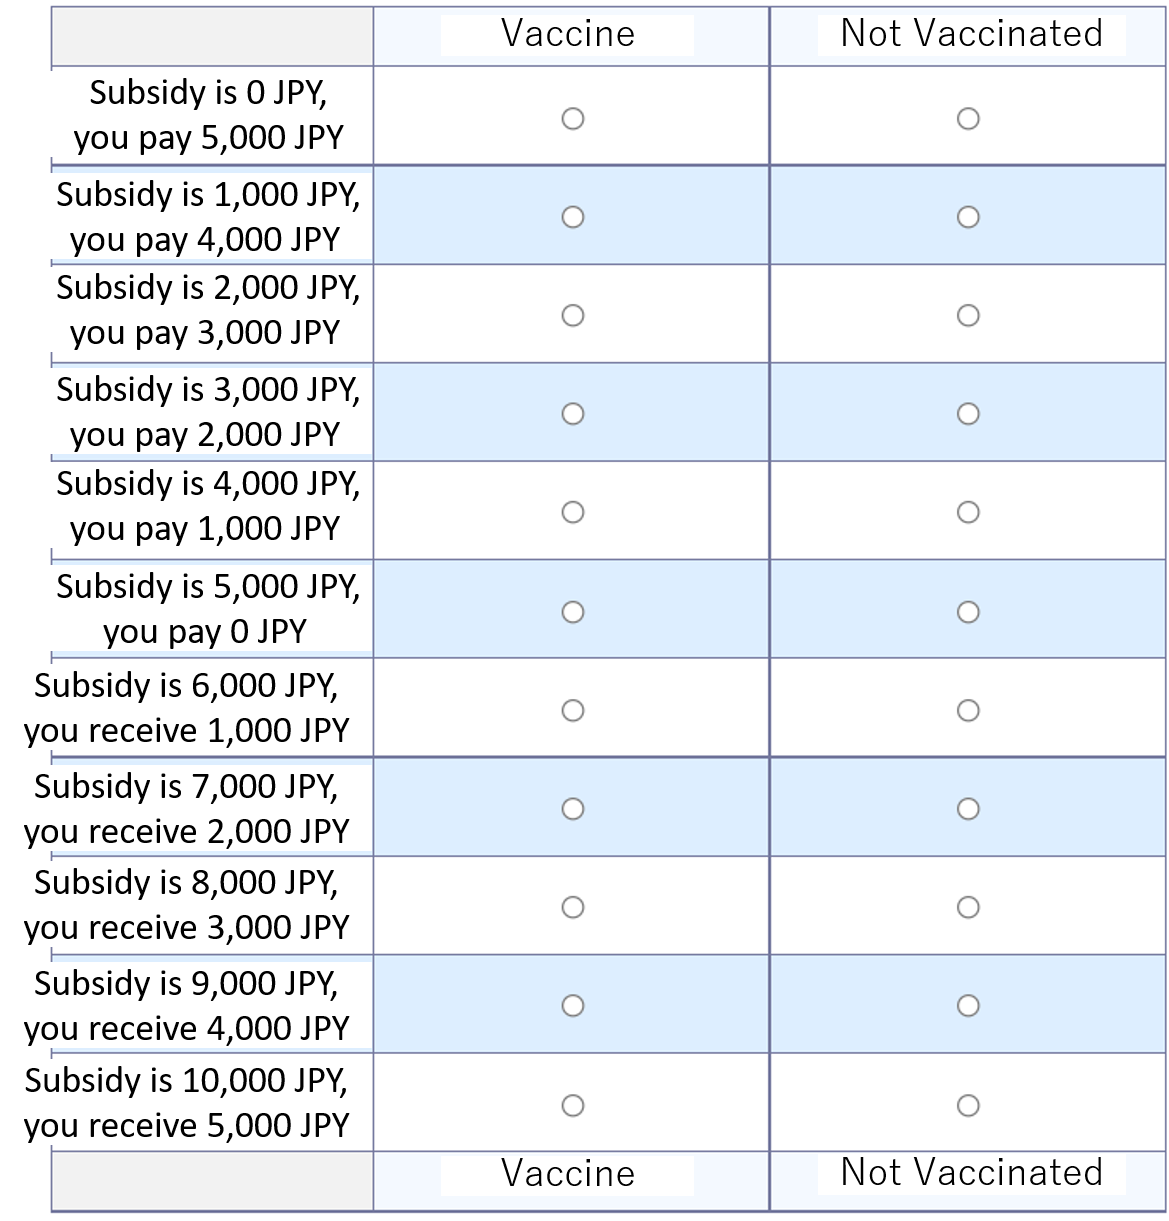
\includegraphics[width=1\linewidth,]{C:/Users/vge00/Desktop/MHLW-Rubella-Project/2020-online-RCT/assets/wtp-question} \caption{Elicitaiton of Willingess-to-Pay for Rubella Vaccination.}\label{fig:wtp-question}
\end{figure}

\begin{figure}[t]
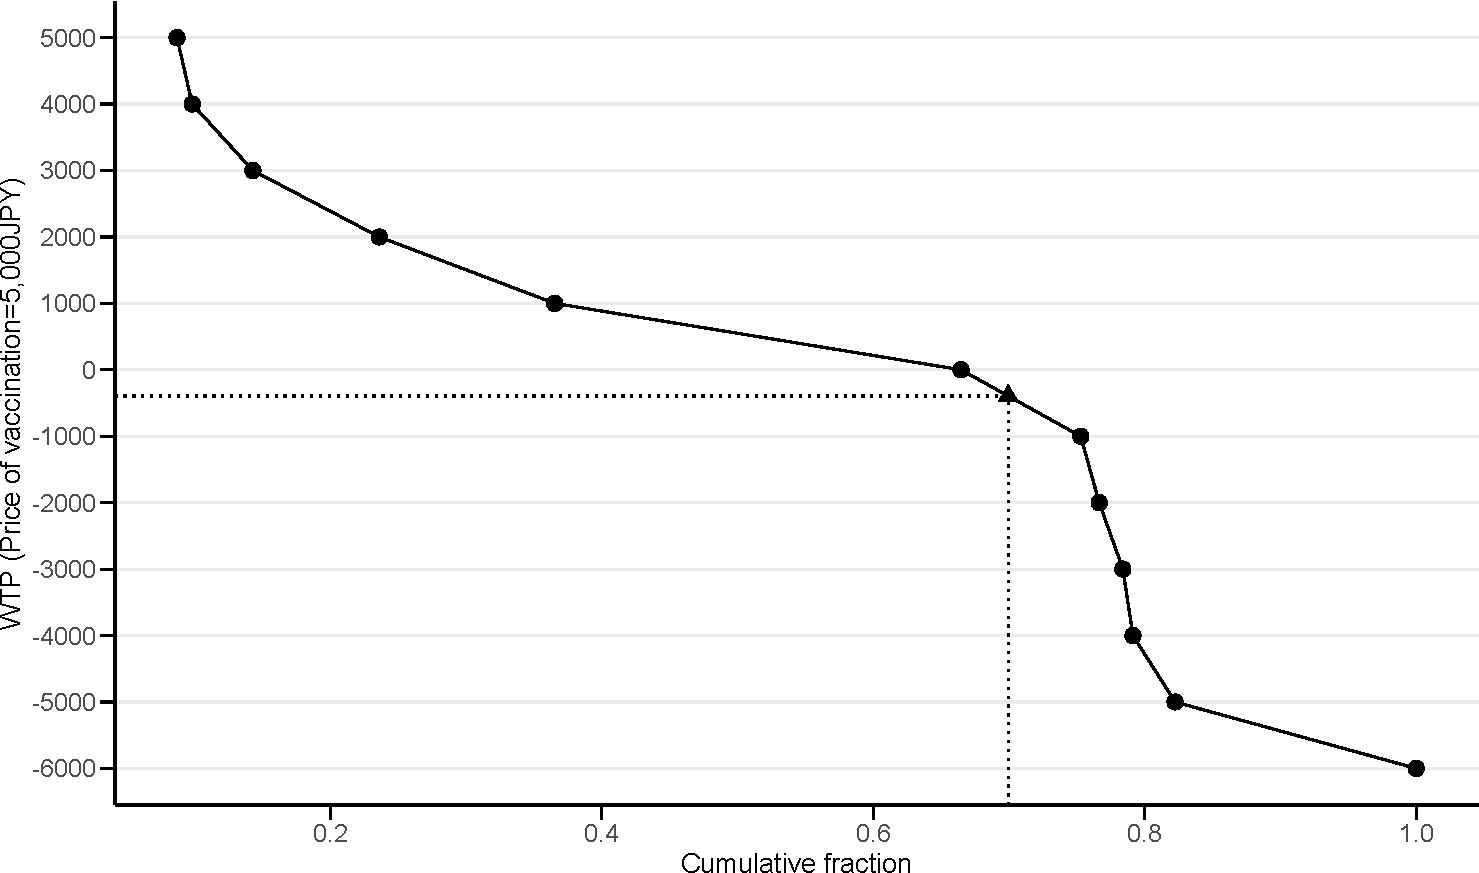
\includegraphics{C:/Users/vge00/Desktop/MHLW-Rubella-Project/2020-online-RCT/publish/appendix_files/figure-latex/demand-vaccine-1} \caption{Demand Curve of Rubella Vaccination among Men for whom Coupons are Automatically Distributed in FY 2019. Data source: wave 2 selection data. Note: Black triangles indicate the sum of the percentage of vaccination when vaccination costs are free and the percentage of antibody test uptake in the MHLW message combined, and the corresponding WTP.}\label{fig:demand-vaccine}
\end{figure}

ナッジ・メッセージの効果を金銭的に評価するために、
我々は風しんワクチンの支払意思額を用いた。
我々は、第1回調査のナッジ・メッセージを示す前に、ワクチン接種の支払意思額を調査した。
支払意思額はMultiple price list法に基づくものである
(調査画面を表\ref{fig:wtp-question}に示した)。

ワクチンの価格は5000円と仮定して、
我々は、自治体の補助金額が\(s_j\)のとき、ワクチン接種をするかどうかを調査した。
補助金額は\(s_j \in \{0, 1000, 2000, \ldots, 10000\}\)とした。
回答者\(i\)が接種すると回答した最低の補助金額を\(s_i^{\text{min}}\)とする。
回答者\(i\)が接種しないと回答した最高の補助金額を\(s_i^{\text{max}}\)とする。
回答者がすべての補助金額\(s_j\)のときの接種しないと回答したならば、\(s_i^{\text{max}} = 10000\)である。
しかしながら、\(s_i^{\text{min}}\)はデータで定義できない。
そこで、\(s_i^{\text{min}} = 11000\)と仮定した。

このとき、回答者\(i\)の支払意思額は
\([5000 - s_i^{\text{min}}, 5000 - s_i^{\text{max}})\)の範囲内で識別される。
したがって、
追加の仮定を置かない限り、ワクチン接種の需要曲線はステップワイズな曲線となり、
メッセージの金銭的価値は範囲で得られる。

メッセージの金銭的価値を点推定するために、
我々は支払意思額が
\([5000 - s_i^{\text{min}}, 5000 - s_i^{\text{max}})\)の範囲で
識別されるとき、
真の支払意思額はその範囲内で一様に分布することを仮定する。
このとき、ステップワイズなワクチン接種の需要曲線は線型補間で表される。
2019年度にクーポン券が自動的に送付され、
第1回調査時点で抗体検査もしくはワクチン接種をしていない男性に限定して、
線型補間された需要曲線を図\ref{fig:demand-vaccine}に示した。

\clearpage

\hypertarget{analysis-to-address-recall-bias-associated-with-self-reporting-of-behavior}{%
\section{Analysis to Address Recall Bias Associated with Self-Reporting of Behavior}\label{analysis-to-address-recall-bias-associated-with-self-reporting-of-behavior}}

\begin{table}[!h]

\caption{\label{tab:act2-coupon1-balance}Balance Test of New Wave 2 Selection Data (Men who automatically received coupon in 2019)}
\centering
\begin{tabular}[t]{l>{\centering\arraybackslash}p{3em}>{\centering\arraybackslash}p{3em}>{\centering\arraybackslash}p{3em}>{\centering\arraybackslash}p{3em}>{\centering\arraybackslash}p{3em}>{\centering\arraybackslash}p{3em}>{\centering\arraybackslash}p{3em}c}
\toprule
\multicolumn{1}{c}{ } & \multicolumn{7}{c}{Treatments} & \multicolumn{1}{c}{ } \\
\cmidrule(l{3pt}r{3pt}){2-8}
  & MHLW (Control) & MHLW (Age) & Altruistic & Selfish & Social comparison & Deadline & Convenient & p-value\\
\midrule
age & 42.869 & 43.063 & 43.099 & 43.016 & 42.948 & 42.901 & 42.893 & 0.948\\
avoid\_crowd & 3.328 & 3.331 & 3.261 & 3.211 & 3.339 & 3.336 & 3.273 & 0.958\\
avoid\_out & 3.082 & 3.047 & 3.028 & 2.805 & 2.896 & 3.038 & 2.926 & 0.509\\
education & 14.598 & 14.457 & 14.592 & 14.236 & 14.130 & 14.267 & 14.603 & 0.530\\
exercise\_w1 & 0.262 & 0.181 & 0.289 & 0.179 & 0.165 & 0.198 & 0.215 & 0.161\\
flushot & 0.238 & 0.268 & 0.211 & 0.130 & 0.148 & 0.244 & 0.215 & 0.040\\
handwash & 3.885 & 3.866 & 3.824 & 3.764 & 3.748 & 3.954 & 3.744 & 0.624\\
health\_check & 0.656 & 0.638 & 0.683 & 0.528 & 0.617 & 0.664 & 0.620 & 0.236\\
income & 556.952 & 652.347 & 611.214 & 625.226 & 564.594 & 588.881 & 640.231 & 0.096\\
married & 0.402 & 0.465 & 0.408 & 0.415 & 0.452 & 0.473 & 0.479 & 0.765\\
noinfo\_income & 0.164 & 0.157 & 0.190 & 0.187 & 0.157 & 0.130 & 0.182 & 0.840\\
temp\_check & 2.180 & 2.260 & 2.380 & 2.179 & 2.226 & 2.145 & 2.157 & 0.735\\
wear\_mask & 2.951 & 3.063 & 3.113 & 3.033 & 2.965 & 3.115 & 3.174 & 0.852\\
\bottomrule
\end{tabular}
\end{table}
\begin{table}[!h]

\caption{\label{tab:act2-coupon0-balance}Balance Test of New Wave 2 Selection Data (Men who need to be processed to receive coupon in 2019)}
\centering
\begin{tabular}[t]{l>{\centering\arraybackslash}p{3em}>{\centering\arraybackslash}p{3em}>{\centering\arraybackslash}p{3em}>{\centering\arraybackslash}p{3em}>{\centering\arraybackslash}p{3em}>{\centering\arraybackslash}p{3em}>{\centering\arraybackslash}p{3em}c}
\toprule
\multicolumn{1}{c}{ } & \multicolumn{7}{c}{Treatments} & \multicolumn{1}{c}{ } \\
\cmidrule(l{3pt}r{3pt}){2-8}
  & MHLW (Control) & MHLW (Age) & Altruistic & Selfish & Social comparison & Deadline & Convenient & p-value\\
\midrule
age & 51.664 & 51.396 & 51.210 & 51.602 & 51.454 & 51.567 & 51.536 & 0.722\\
avoid\_crowd & 3.307 & 3.378 & 3.429 & 3.250 & 3.306 & 3.296 & 3.455 & 0.354\\
avoid\_out & 2.903 & 2.917 & 2.919 & 2.884 & 2.825 & 2.966 & 2.982 & 0.848\\
education & 14.542 & 14.652 & 14.533 & 14.833 & 14.576 & 14.609 & 14.378 & 0.589\\
exercise\_w1 & 0.160 & 0.196 & 0.248 & 0.231 & 0.188 & 0.206 & 0.216 & 0.304\\
flushot & 0.223 & 0.243 & 0.200 & 0.264 & 0.284 & 0.223 & 0.248 & 0.453\\
handwash & 3.803 & 3.883 & 3.900 & 3.778 & 3.817 & 3.833 & 3.892 & 0.827\\
health\_check & 0.634 & 0.661 & 0.690 & 0.685 & 0.651 & 0.670 & 0.649 & 0.872\\
income & 709.184 & 711.202 & 688.773 & 673.323 & 645.225 & 712.130 & 713.246 & 0.326\\
married & 0.588 & 0.578 & 0.624 & 0.662 & 0.603 & 0.554 & 0.608 & 0.337\\
noinfo\_income & 0.185 & 0.165 & 0.129 & 0.111 & 0.157 & 0.163 & 0.212 & 0.076\\
temp\_check & 2.139 & 2.248 & 2.210 & 2.083 & 2.192 & 2.086 & 2.270 & 0.490\\
wear\_mask & 3.071 & 3.191 & 3.157 & 3.148 & 2.961 & 2.966 & 3.068 & 0.447\\
\bottomrule
\end{tabular}
\end{table}

ここでは、第2回調査の抗体検査の受検行動やワクチン接種行動の回答に
想起バイアスが伴うことを考慮した分析を行う。
第2回調査はそれぞれの行動を第1回調査以前に行ったかどうかを調査している。
この時期の回答に想起バイアスが伴うならば、
本論の分析のように第2回調査で第1回調査以前に行動したと回答した人を除くべきではない。
そこで、我々は第2回調査の行動の回答に想起バイアスが伴うことを仮定して、
第1回調査の調査ですでに抗体検査もしくはワクチン接種を受けた男性だけを除いて、
ナッジ・メッセージの行動に対する効果を推定する(wave 1 selection dataと同じ基準)。
したがって、
第2回調査で第1回調査以前に抗体検査もしくはワクチン接種を受けたと回答した人はサンプルに含まれている。

本論と同様に、
我々は2019年度にクーポン券を自動的に受け取っているかどうかでサンプルを分割して、
サブサンプルを用いてナッジ・メッセージの効果を推定する。
表\ref{tab:act2-coupon1-balance}と
表\ref{tab:act2-coupon0-balance}は共変量のバランステストの結果であり、
回答者の観察可能な特徴は群間でシステマティックに異ならないことを示している。

検定力80\%・有意水準5\%を保つために必要な効果の規模を計算したところ、
2019年度にクーポン券が自動で送付される男性のサブサンプルを用いる場合、少なくとも
6.8
\%ポイントの差が必要である。
2019年度ではクーポン券を受け取るために手続きが必要な男性のサブサンプルを用いる場合、少なくとも
5.2
\%ポイントの差が必要である。

アウトカム変数の定義も本論のものから変更する。
本論では、第1回調査以降に抗体検査を受検したら1を取るアウトカム変数と
第1回調査以降に抗体検査を受検し、ワクチンによって抗体を新たに獲得したら1を取るダミー変数でを用いた。
対して、この補論では、
第2回調査で時期に関わらず抗体検査を受検したと回答したら1を取るダミー変数と
第2回調査で時期に関わらず抗体検査を受検し、
時期に関わらずワクチンによって抗体を獲得したら1を取るダミー変数である。

\begin{figure}[t]
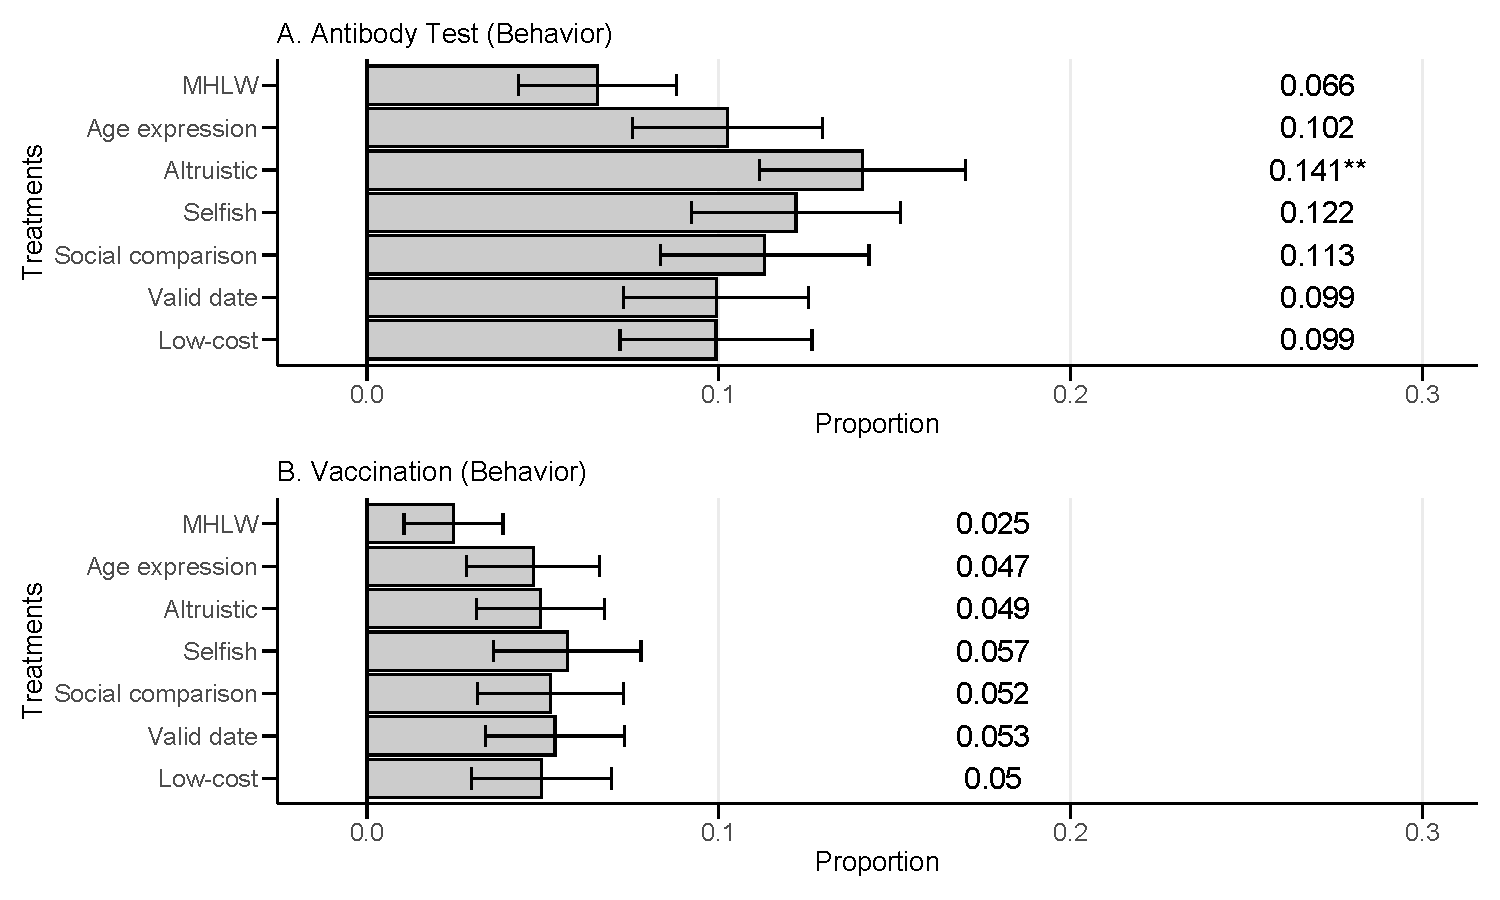
\includegraphics{C:/Users/vge00/Desktop/MHLW-Rubella-Project/2020-online-RCT/publish/appendix_files/figure-latex/act2-coupon1-ttest-1} \caption{Effect of Text-Based Nudges on Behavior among Men for whom Coupons are Automatically Distributed in FY 2019 (N = 881). Data source: new wave 2 selection data. Note: Numbers in the figure indicate the proportion of each group. Error bars indicate standard error of the mean. Asterisks are p-values for t-tests of the difference in means from the MHLW message group: * p < 0.1, ** p < 0.05, *** p < 0.01.}\label{fig:act2-coupon1-ttest}
\end{figure}
\begin{figure}[t]
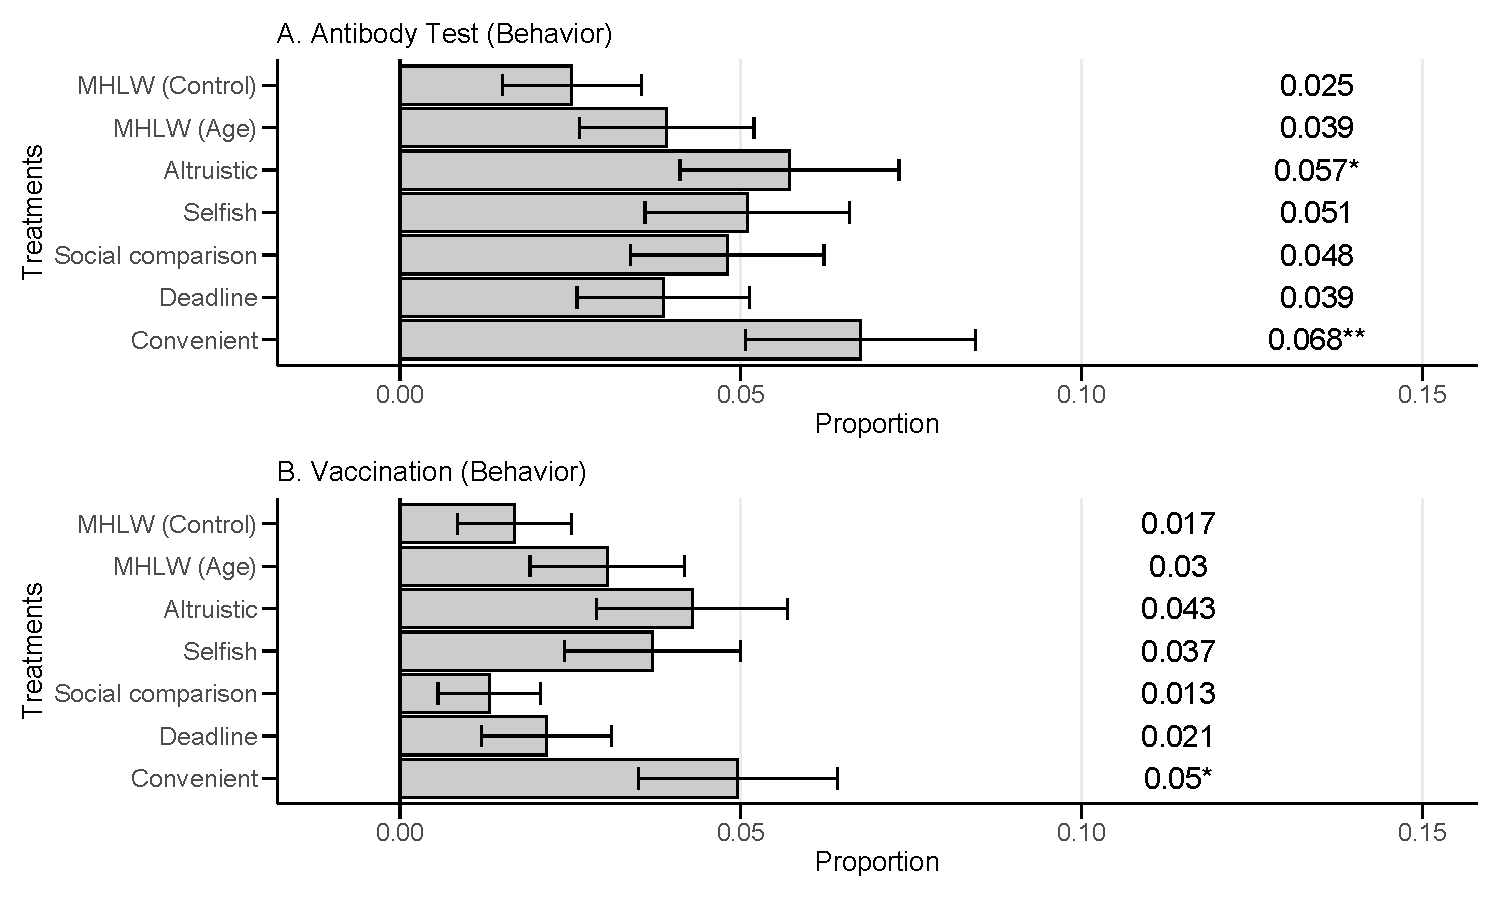
\includegraphics{C:/Users/vge00/Desktop/MHLW-Rubella-Project/2020-online-RCT/publish/appendix_files/figure-latex/act2-coupon0-ttest-1} \caption{Effect of Text-Based Nudges on Behaviors among Men Who Needed Costly Procedures to Receive Coupons in FY 2019 (N = 1,578). Data source: new wave 2 selection data. Note: Numbers in the figure indicate the proportion of each group. Error bars indicate standard error of the mean. Asterisks are p-values for t-tests of the difference in means from the MHLW message group: * p < 0.1, ** p < 0.05, *** p < 0.01.}\label{fig:act2-coupon0-ttest}
\end{figure}

2019年度にクーポン券を自動的に受け取った男性に限定して、
我々は各介入群の抗体検査受検率(パネルA)とワクチン接種率(パネルB)を
図\ref{fig:act2-coupon1-ttest}に示した。
その結果、利他強調メッセージは厚労省メッセージよりも抗体検査受検率が高い。
厚労省メッセージの抗体検査受検率は6.6\%であるのに対し、
利他強調メッセージの抗体検査受検率は14.1\%である。
したがって、厚労省メッセージと比較して、
利他強調メッセージは抗体検査の受検率を7.5\%ポイント高めていて、
これは統計的に5\%水準で有意である。
この効果の規模は本論の結果と一致している。
また、利他強調メッセージのワクチン接種率に対する効果は統計的に非有意である。

2019年度にクーポン券を受け取るためにはコストのかかる手続きが必要な男性に限定して、
我々は各介入群の抗体検査受検率(パネルA)とワクチン接種率(パネルB)を
図\ref{fig:act2-coupon0-ttest}に示した。
その結果、利他強調メッセージと低コストメッセージは厚労省メッセージよりも抗体検査の受検率を高めていて、
低コストメッセージのみが厚労省メッセージよりもワクチン接種率を高めている。
厚労省メッセージの抗体検査の受検率は2.5\%であり、
利他強調メッセージと低コストメッセージの受検率はそれぞれ5.7\%と6.8\%である。
したがって、利他強調メッセージと低コストメッセージの抗体検査の受検率に対する効果はそれぞれ
3.2\%ポイント・4.3\%ポイントであり、
これらは統計的に有意である。
また、厚労省メッセージのワクチン接種率は1.7\%であり、
低コストメッセージの受検率は5\%である。
したがって、低コストメッセージのワクチン接種率に対する効果は3.3\%ポイントであり、
これは統計的に10\%水準で有意である。

\begin{table}

\caption{\label{tab:act2-reg}Linear Probability Model of Behaviors Using New Wave 2 Selection Data}
\centering
\begin{threeparttable}
\begin{tabular}[t]{lcc}
\toprule
\multicolumn{1}{c}{ } & \multicolumn{1}{c}{Antibody Test} & \multicolumn{1}{c}{Vaccination} \\
\cmidrule(l{3pt}r{3pt}){2-2} \cmidrule(l{3pt}r{3pt}){3-3}
  & (1) & (2)\\
\midrule
MHLW (Age) & 0.010 & 0.012\\
 & (0.017) & (0.014)\\
Altruistic & 0.028 & 0.023\\
 & (0.019) & (0.016)\\
Selfish & 0.020 & 0.019\\
 & (0.018) & (0.015)\\
Social comparison & 0.020 & -0.005\\
 & (0.018) & (0.011)\\
Deadline & 0.013 & 0.005\\
 & (0.016) & (0.013)\\
Convenient & 0.041** & 0.031*\\
 & (0.020) & (0.017)\\
Coupon & 0.019 & -0.014\\
 & (0.028) & (0.021)\\
Coupon×Age expression & 0.025 & 0.010\\
 & (0.038) & \vphantom{1} (0.027)\\
Coupon×Altruistic & 0.046 & 0.000\\
 & (0.041) & (0.028)\\
Coupon×Selfish & 0.042 & 0.015\\
 & (0.041) & (0.029)\\
Coupon×Social comparison & 0.031 & 0.032\\
 & (0.041) & (0.027)\\
Coupon×Valid date & 0.019 & 0.023\\
 & (0.038) & (0.027)\\
Coupon×Low-cost & -0.006 & -0.006\\
 & (0.040) & (0.029)\\
\midrule
Num.Obs. & 2459 & 2459\\
R2 & 0.096 & 0.052\\
R2 Adj. & 0.086 & 0.042\\
Covariates & X & X\\
\bottomrule
\end{tabular}
\begin{tablenotes}
\item Note: * p < 0.1, ** p < 0.05, *** p < 0.01. We use robust standard errors. We also control for covariates obtained in wave 1 and 2. The list of covariates is presented in Table \ref{tab:covlist}.
\end{tablenotes}
\end{threeparttable}
\end{table}
\begin{table}

\caption{\label{tab:act2-reg-ftest}Effects of Text-Based Nudges on Behaviors Using Linear Probability Model Estimates (Data: New Wave 2 Selection Data)}
\centering
\begin{tabular}[t]{>{\raggedright\arraybackslash}p{5em}lcccccc}
\toprule
\multicolumn{2}{c}{ } & \multicolumn{3}{c}{Antibody Test} & \multicolumn{3}{c}{Vaccination} \\
\cmidrule(l{3pt}r{3pt}){3-5} \cmidrule(l{3pt}r{3pt}){6-8}
How to get coupons & Text-based nudges & estimate & std.error & p.value & estimate  & std.error  & p.value \\
\midrule
Costly procedure & MHLW (Age) & 0.010 & 0.017 & 0.530 & 0.012 & 0.014 & 0.404\\
 & Altruistic & 0.028 & 0.019 & 0.146 & 0.023 & 0.016 & 0.152\\
 & Selfish & 0.020 & 0.018 & 0.270 & 0.019 & 0.015 & 0.213\\
 & Social comparison & 0.020 & 0.018 & 0.275 & -0.005 & 0.011 & 0.668\\
 & Deadline & 0.013 & 0.016 & 0.436 & 0.005 & 0.013 & 0.688\\
 & Convenient & 0.041 & 0.020 & 0.039 & 0.031 & 0.017 & 0.065\\
Automatic receiving & MHLW (Age) & 0.035 & 0.035 & 0.308 & 0.022 & 0.023 & 0.354\\
 & Altruistic & 0.074 & 0.036 & 0.043 & 0.023 & 0.023 & 0.306\\
 & Selfish & 0.062 & 0.037 & 0.088 & 0.034 & 0.025 & 0.175\\
 & Social comparison & 0.051 & 0.037 & 0.166 & 0.027 & 0.025 & 0.278\\
 & Deadline & 0.032 & 0.034 & 0.347 & 0.028 & 0.024 & 0.246\\
 & Convenient & 0.035 & 0.035 & 0.322 & 0.025 & 0.024 & 0.296\\
\bottomrule
\end{tabular}
\end{table}

サブサンプルで推定されたナッジ・メッセージの効果は
クーポン券が自動的に送付されるかどうかだけでなく、
年齢の違いの影響を受けるので、
我々はこの問題を排除するために線形確率モデルを推定した。
基本的に、二群の平均値の差の検定の結果と整合的である。
それに加えて、表\ref{tab:act2-reg-ftest}より、
2019年度にクーポン券を自動的に受け取った男性における
利己強調メッセージの抗体検査受検率に対する効果は6.2\%ポイントであり、
これは統計的に10\%水準で有意である。
また、2019年度にクーポン券を受け取るためにはコストのかかる手続きが必要な男性における
利他強調メッセージの抗体検査受検率に対する効果は
効果の規模が変化していないにも関わらず、統計的に非有意である。
さらに、表\ref{tab:act2-reg}より、
クーポン券を自動的に送付されるかどうかによる
ナッジ・メッセージの効果の異質性は統計的に非有意である。

\begin{table}

\begin{threeparttable}
\caption{\label{tab:tester2-move}Movement of Antibody Test Takers (Data: New Wave 2 Selection Data)}
\centering
\fontsize{9}{11}\selectfont
\begin{tabular}[t]{>{\raggedright\arraybackslash}p{9em}>{\centering\arraybackslash}p{5em}>{\centering\arraybackslash}p{5em}>{\centering\arraybackslash}p{5em}>{\centering\arraybackslash}p{5em}>{\centering\arraybackslash}p{5em}>{\centering\arraybackslash}p{5em}}
\toprule
\multicolumn{1}{c}{ } & \multicolumn{3}{c}{w/ receiving coupon automatically} & \multicolumn{3}{c}{w/o receiving coupon automatically} \\
\cmidrule(l{3pt}r{3pt}){2-4} \cmidrule(l{3pt}r{3pt}){5-7}
Text-based nudge & Antibody test & Negative test result & Vaccination & Antibody test  & Negative test result  & Vaccination \\
\midrule
MHLW (Control) & 8 & 3 & 3 & 6 & 4 & 4\\
MHLW (Age) & 13 & 6 & 6 & 9 & 9 & 7\\
Altruistic & 20 & 8 & 7 & 12 & 9 & 9\\
Selfish & 15 & 7 & 7 & 11 & 8 & 8\\
Social comparison & 13 & 7 & 6 & 11 & 5 & 3\\
Deadline & 13 & 7 & 7 & 9 & 6 & 5\\
Convenient & 12 & 8 & 6 & 15 & 13 & 11\\
Fisher's exact test (p-value) &  & 0.83 & 0.76 &  & 0.12 & 0.30\\
\bottomrule
\end{tabular}
\begin{tablenotes}
\small
\item [] Note: Limiting our sample to antibody test takers, we tested the null hypothesis that the number of negative antibody tests does not differ between intervention groups with Fisher's exact test. Also, restricting the sample to negative individuals, we tested the null hypothesis that the number of vaccinations would not differ between intervention groups with a Fisher's exact test.
\end{tablenotes}
\end{threeparttable}
\end{table}

表\ref{tab:tester2-move}は各介入群の抗体検査の受検者数・陰性件数・ワクチン接種件数を示した。
本論と同様に、
クーポン券を自動的に受け取ったかどうか・介入群に関わらず、
抗体検査の結果が陰性である人のほとんどがワクチンを接種している。
よって、ワクチン接種率に対するナッジ・メッセージの効果は介入群の陰性比率に強く依存している。
事実、手続きが必要な男性に限定したとき、
低コストメッセージの陰性比率は87\%(\(=13/15\))と非常に高い。
その結果、低コストメッセージはワクチン接種率に統計的に有意な効果を持っている。
しかしながら、介入群間の陰性比率のバラツキは統計的な誤差である可能性が高い。
我々は抗体検査の受検者をクーポン券が自動的に送付されるかどうかで分割し、
抗体検査の陰性件数が介入群間で同じであるという帰無仮説をフィッシャーの正確検定で検証した。
その結果、二つのサブサンプルで帰無仮説を棄却できない。

\begin{figure}[t]
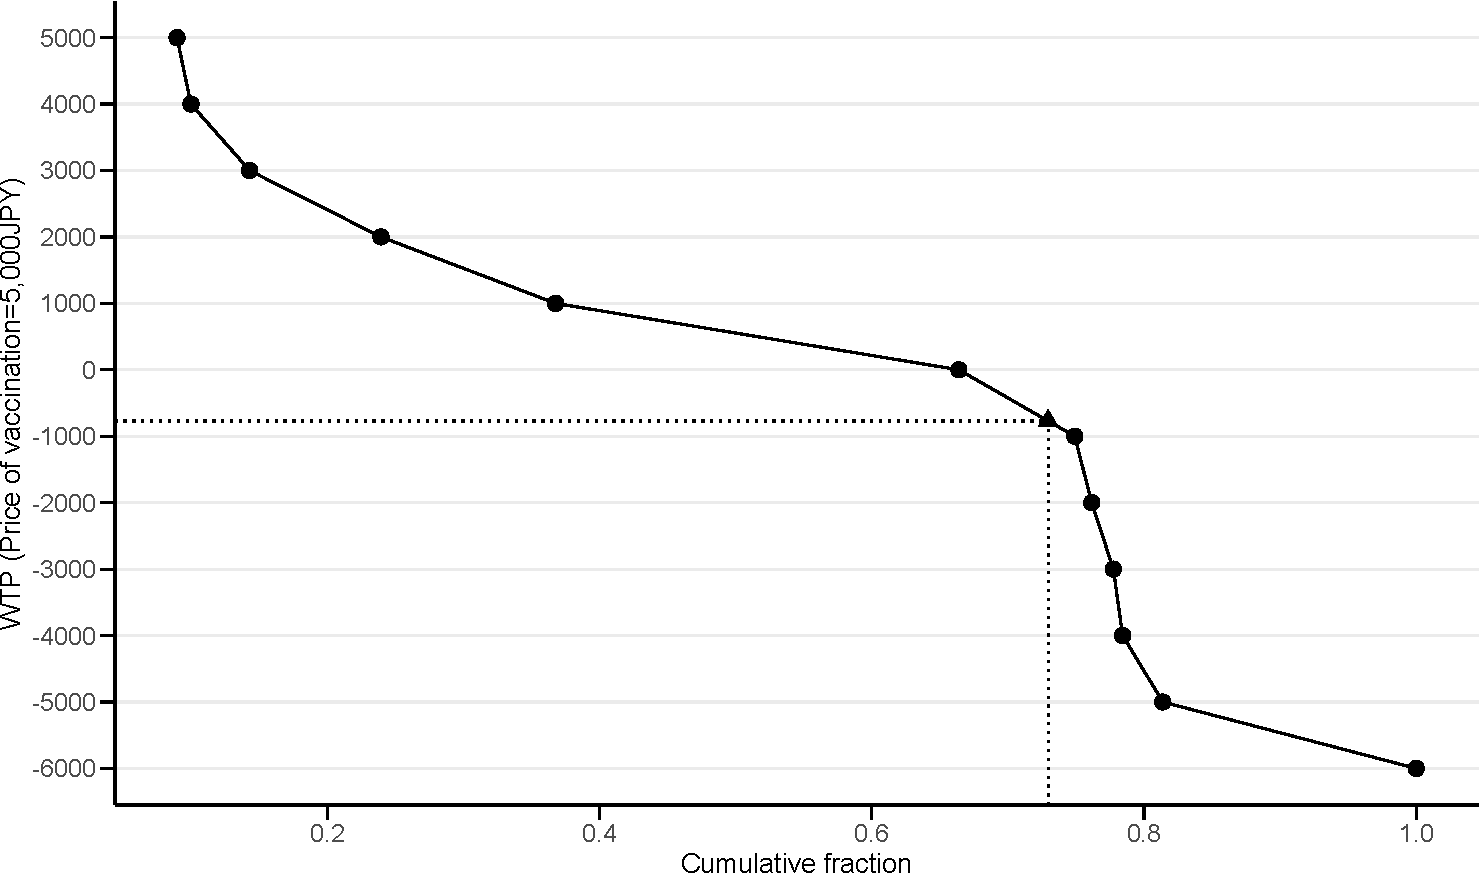
\includegraphics{C:/Users/vge00/Desktop/MHLW-Rubella-Project/2020-online-RCT/publish/appendix_files/figure-latex/demand2-vaccine-1} \caption{Demand Curve of Rubella Vaccination among Men for whom Coupons are Automatically Distributed in FY 2019. Data source: new wave 2 selection data. Note: Black triangles indicate the sum of the percentage of vaccination when vaccination costs are free and the percentage of antibody test uptake in the MHLW message combined, and the corresponding WTP.}\label{fig:demand2-vaccine}
\end{figure}

2019年度にクーポン券を自動的に受け取る人へのナッジ・メッセージの効果を
金銭的な価値で評価することを試みる。
本論で示した方法を用いて、図\ref{fig:demand2-vaccine}に
2019年度に自動的にクーポン券を受け取る人に限定した、風しんワクチン接種の需要曲線を示した。
ワクチン接種が0円で供給されているとき、均衡接種割合は0.664である。

\begin{table}

\caption{\label{tab:economic-value2}Estimated Monetary Value of Text-Based Nudges}
\centering
\resizebox{\linewidth}{!}{
\fontsize{9}{11}\selectfont
\begin{threeparttable}
\begin{tabular}[t]{lcccccc}
\toprule
\multicolumn{3}{c}{ } & \multicolumn{2}{c}{Monetary value (JPY)} & \multicolumn{2}{c}{Monetary value (USD)} \\
\cmidrule(l{3pt}r{3pt}){4-5} \cmidrule(l{3pt}r{3pt}){6-7}
Text-based nudge & Size of effect & Baseline + size of effect & pp & total & pp  & total \\
\midrule
MHLW (Age) & 0.037 & 0.766 & 1528.377 & 8.085 & 13.894 & 73.501\\
Altruistic & 0.075 & 0.805 & 3925.285 & 20.765 & 35.684 & 188.771\\
Selfish & 0.056 & 0.786 & 3285.074 & 17.378 & 29.864 & 157.982\\
Social comparison & 0.047 & 0.777 & 2200.534 & 11.641 & 20.005 & 105.826\\
Deadline & 0.034 & 0.763 & 1331.690 & 7.045 & 12.106 & 64.042\\
Convenient & 0.034 & 0.763 & 1327.720 & 7.024 & 12.070 & 63.851\\
\bottomrule
\end{tabular}
\begin{tablenotes}
\item Note: Effect is the size of effect of each text-based nudge on antibody test. Baseline is the sum of the rate of antibody test in the control and the vaccination rate when the vaccine is free The monetary value is the amount per person (pp) and the total amount (total) multiplied by the number of people who received the coupon in 2019 but did not use it until January, 2020. We valued the monetary value in Japanese Yen (JPY) and US Dollars (USD) (1USD = 110JPY). The unit of monetary value per person is 1 JPY and 1 USD, respectively. The unit of total monetary value is 1 billion JPY and 1 million USD, respectively.
\end{tablenotes}
\end{threeparttable}}
\end{table}

抗体検査の受検確率をナッジ・メッセージの効果量として用いて、
表\ref{tab:economic-value2}にメッセージの金銭的価値を示した。
第2列は図\ref{fig:act2-coupon1-ttest}のパネルAで示した比率を示している。
第3列はベースラインの均衡接種割合からメッセージの効果分だけ増やしたときの接種割合を示している。
第4列はそのその接種割合と対応する自治体の追加的な補助金額であり、
これがメッセージの一人当たりの金銭的価値である。
アメリカドルに換算した価値は第6列に示した。
利他強調メッセージの一人当たりの金銭的価値は約3900円(約35ドル)である。
第5列はメッセージの一人当たりの金銭的価値を
2019年度にクーポン券が発行されたにもかかわらず、
1月時点で抗体検査のクーポン券を利用していない人口で掛けた
メッセージの金銭的価値の総額を示している。
アメリカドルに換算した価値は第7列に示している。
利他強調メッセージの金銭的価値の総額はそれぞれ200億円である。

\end{document}
